\documentclass[conference]{IEEEtran}
\usepackage[justification=centering]{caption}
\usepackage{blindtext, graphicx}
\usepackage{float}

\begin{document}
\title{TeamFinder: An Application for Building Skill Based Teams}


\author{\IEEEauthorblockN{Michael Goff\IEEEauthorrefmark{1},
Shashank Jha\IEEEauthorrefmark{2},
Jingjuan Deng\IEEEauthorrefmark{3} and
Bhaskar Sinha\IEEEauthorrefmark{4}}
\IEEEauthorblockA{Department of Computer Science, North Carolina State University, \\
Raleigh, North Carolina 27606\\ 
Email: \IEEEauthorrefmark{1}magoff2@ncsu.edu \\
\IEEEauthorrefmark{2}sjha5@ncsu.edu \\
\IEEEauthorrefmark{3}jdeng8@ncsu.edu \\
\IEEEauthorrefmark{4}bsinha@ncsu.edu}}


% make the title area
\maketitle

\section{Collections}


\section{Anonymization}
In order to protect the identity of our peers we anonomized the data we pulled from the various GitHub repositories. The anonomization was performed both on the group name and the users themselves so no connection could be made back to the individuals. When gathering data each new group that was added to our databases was assigned an id number. Additionally each new user that appeared in an interaction was also assigned an id number. With personal data pulled away we can be assured that it is safe to objectively analyze the repository data without fear of offending any particular group. 

\section{Data Summary}
We have pulled data across all of the groups in the software engineering course but we decided to focus on the 3 groups with the most active repository. Below is a table of summary information about each team. 


\begin{tabular}{c|c|c|c|c}
    Team & Commits &  Issues & Milestones & Comments \\
    1 & 202 & 49 & 8 & 140 \\
    2 & 138 & 27 & 5 & 13 \\
    3 & 60 & 32 & 4 & 72 \\
\end{tabular}

It is important to note that the professor asked students to try to use GitHub as their main source of communication throughout the semester in order to generate data for this project. However, upon inspection of the data it seems that some groups talked much more than others. Team 1 maintained a high number across the board for the project by maintaining a high frequency of commits at 202 where the other groups did not keep such a high number. Perhaps team 1 prioritized frequent smaller changes while other teams preferred to make large changes at once. Another important area to judge the active level of the repository are comments. A repository with a lot of comments would imply that there was enough communication to successfully get a job done. Once again team 1 had the most with 140 comments. Team 2 had a surprising 13 comments, which almost surely implies that the team was communicating mainly outside of GitHub. The number of issues were fairly similar among teams, with 1 having the most and 2 having the least. It could be a case of breaking issues down into smaller pieces rather than big features to implement. 

\section{Data Samples}

\section{Features}
This section will describe the various metrics we want to observe about a team to form a hypothesis about their performance. If all of these different symptoms look like they are in good shape then the project is probably going along smoothly. 

\subsection{Comments per Issue}
One feature we were interested in looking into was the number of comments per issue. The reason we wanted to look at this issue was to judge the level of collaboration between team members. If there were few comments then problems may not have been resolved in a proper manner. When paired with the time issues remain open we can gather even more insight. For instance, if an issue is open with one or less comments over an extended period of time then we can see that there is a problem with development. Another possible situation could be that the item is not a high priority, though a good team would probably leave a comment or label to make it as such. 

\subsection{Issue Duration}
Another important feature on a repository is the duration an issue remains open. Issues that have not been resolved for a long period of time may indicate features that have not been properly developed or bugs that have persisted for too long in the system. If these types of situations are not cleared up in a timely manner it can have a cumulative effect on an application. We hope to find that issues are resolved within a week of being found. This would indicate an active developer community that can quickly resolve errors in a system. If issues are left open for a longer period of time then the developers are not keeping up with the problems in the application which, over time, may lead to larger problems within the system. 

\subsection{Comments vs Issue Duration}
When it comes to issues that remained open for a longer period of time we were considering why it would be the case. One explanation could be it was remaining open as a way to discuss the solution to that issue before it was actually fixed. As a result, we wanted to graph the relationship between comments and issue duration. The idea is if the issue is open for longer there should be more comments on it. 

\subsection{Issue open time outside of milestone deadline}
On GitHub, issues are usually assigned to milestones. This allows developers to group similar functionality together for a release. One aspect that observes how issues and milestones are connected is whether the issue was closed before the deadline of the milestone. We predict that a good group will have most of their issues close before the due date for the milestone. 

\subsection{Project Milestones Timeline}
On GitHub, milestones can be set for projects which mark a significant stage in the project and users can also set due dates for those milestones, also, close date are noted for every milestones. Users can set multiple milestones by diving the project into significant chunks. In general, there is no correlation between how many milestones the project has and the success of the project but every project has many small deliverables and landmarks and if they are broken down into milestones it becomes easy to track the progress of the project. We anticipate that if a project has multiple milestones, most of which are closed within the due date, could lead to the success of the project.

\subsection{User Issue Comments}
Issues can be linked to a milestone and users can also make comments on those issues. Our understanding is that if users make comments on issues, it shows their participation on resolving the issue. We predict that for a successful project, the comments on issues would be made by a majority of the users.

\subsection{Percent Commits by User}
On GitHub, the commits made by each user for a project can be observed. The number of commits to a project by a user represents a direct correlation with the contribution of that user on the project. We reckon that a good project will have almost equal contribution from each member, in other words, the percent of commits should be almost equally divided among users.

\section{Results}
\subsection{Comments per Issue}
When pulling the number of comments per issue on the same teams we found that the average number of comments were surprisingly low across the teams as shown in figure \ref{comments_issue}. When looking at the box and whisker plot of the teams there was a telling spread of different stories across the teams. For example the majority of team 1's issues had less than 7 comments. One explanation to the lack of comments was that issues were resolved quickly and closed. Team 1 also had a lot of outlier issues that had a lot more comments than the rest of the issues. The deviance of the norm on these issues could be attributed to discussion threads that take place on the issues. It is common among groups to have a place to discuss next steps or debate over a new feature or design idea.

\begin{figure}[H]
    \centering
    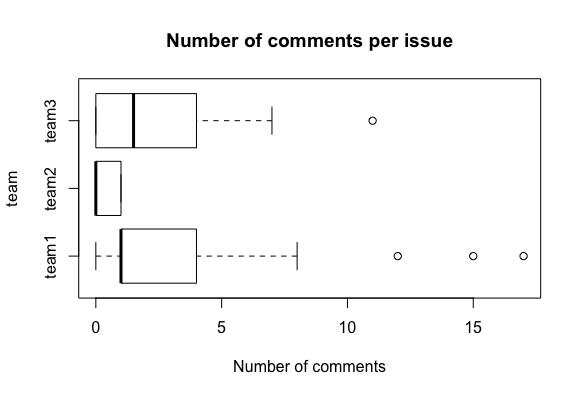
\includegraphics[width=9cm]{../AprilProject/pic/comments_per_issue.png}
    \caption{Comments per Issue across Teams}
    \label{comments_issue}
\end{figure}

The box and whisker plot did not do a great job of painting a complete picture so we decided to capture the comments per issue in the form of a distribution graph instead. Figure \ref{comments_issue_total} is a distribution of the number of comments on each issue for all of the teams in the class. We quickly noticed that the vast majority of issues have 0 comments on them. Perhaps in these situations people marked the issues that needed done after they were discussed in person so there was no need to comment on them. On the other hand the description in the issue may have been clear enough that no other comments needed to be made. Regardless, the majority of the teams hardly used any comments on their issues. 

\begin{figure}[H]
    \centering
    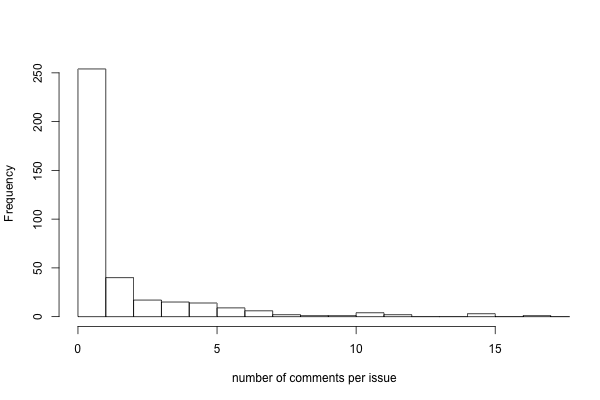
\includegraphics[width=9cm]{../AprilProject/pic/distribution/comment_per_issue_distribution_total.png}
    \caption{Distribution of comments per issue across all teams}
    \label{comments_issue_total}
\end{figure}

Team 1's distribution, shown in figure \ref{comments_issue_team1}, largely reflects the total distribution in shape. However, team 1 had a few more issues that had a couple of comments. It seems that team 1 had a bit more active discussion on a number of issues, but the vast majority of the issues still had zero comments.

\begin{figure}[H]
    \centering
    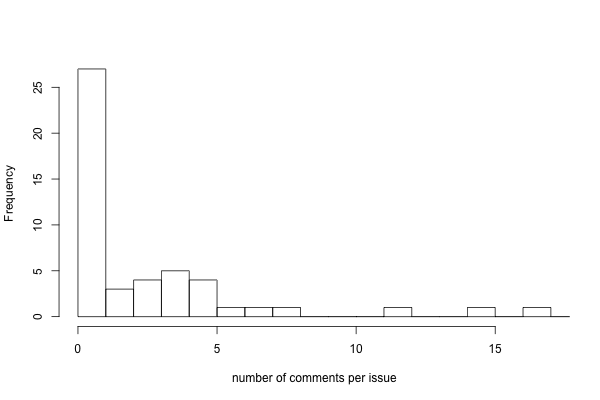
\includegraphics[width=9cm]{../AprilProject/pic/distribution/comment_per_issue_distribution_team1.png}
    \caption{Distribution of comments per issue for team 1}
    \label{comments_issue_team1}
\end{figure}

When we created the graph for team 2's data we discovered that team 2 had not made more than one comment on any of their issues at all. There was pretty much no discussion to be had on the GitHub repository for team 2. We are finding this time and time again through out metrics. 

\begin{figure}[H]
    \centering
    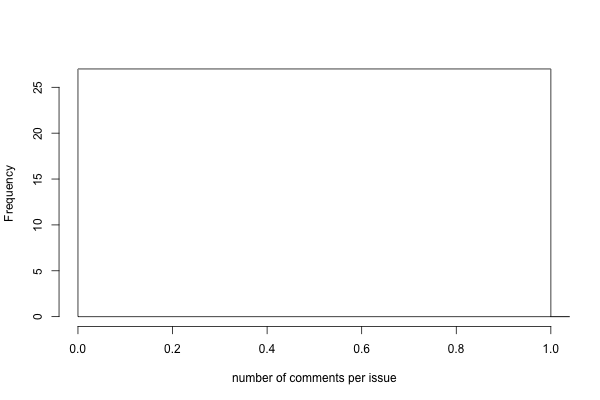
\includegraphics[width=9cm]{../AprilProject/pic/distribution/comment_per_issue_distribution_team2.png}
    \caption{Distribution of comments per issue for team 2}
    \label{comments_issue_team2}
\end{figure}

Finally, team 3 was much more like the overall distribution as well, as seen in figure \ref{comments_issue_team3}. Team 3 had a stronger presence of one or a few comments compared to their majority of zero comment issues. We think that there was just some confirmation comments on the issues as they were assigned that would make up for this difference. 

\begin{figure}[H]
    \centering
    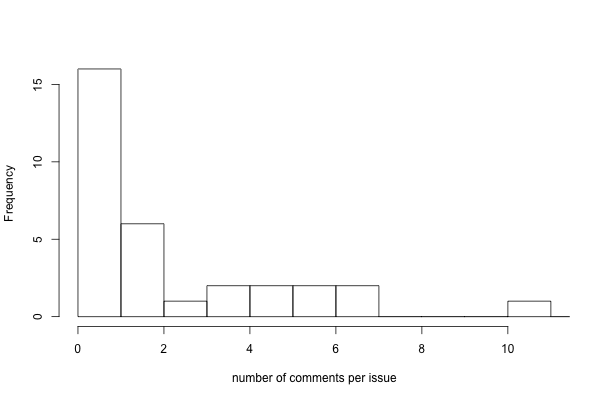
\includegraphics[width=9cm]{../AprilProject/pic/distribution/comment_per_issue_distribution_team3.png}
    \caption{Distribution of comments per issue for team 3}
    \label{comments_issue_team3}
\end{figure}

Judging across all of the groups team 1 and 3 look the healthiest and team 2 looks like it is in trouble. The number of comments average is very close to zero and they did not have a single issue that contained more than 1 comment. The lack of discussion on issues indicates that there was a poor level of communication across the team. There could be some explanations to the lack of comments on issues, like another external communication channel outside of GitHub. It is possible that team 2 mainly communicated on the side and did not feel the need to document everything in issues. While this feature alone is not enough to indicate a bad team, when combined with other bad signs it could paint a more complete picture. 

\subsection{Issue Duration}
Across the teams the results were somewhat surprising when it came to issue duration, seen in figure \ref{issue_duration}. We predicted that issues would on average be open for about a week, which turned out to be mostly true except for team 3. Team 2 had an average open time of only a couple of days while team 1 had issues open for an average of 6 days. There are a lot of outlier issues on this figure though. When it comes to outlier issues, team 1 is the biggest offender. They had 7 issues that were open 30 days or longer. Surprisingly, the number of outliers did not seem to pull the average close time past a week so they must have had plenty of issues that were quickly resolved as well. 

\begin{figure}[H]
    \centering
    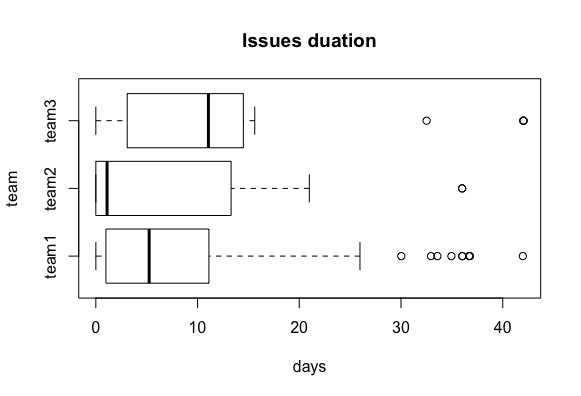
\includegraphics[width=9cm]{../AprilProject/pic/issues_duration.png}
    \caption{Duration of Issues}
    \label{issue_duration}
\end{figure}

With teams 1 and 2 quickly resolving issues it seems to indicate that they have healthier projects when it comes to turnaround on issues. Team 3 had the biggest problem with average duration. They had issues open an average of a week and a half. Often, just looking at averages is not enough when it comes to something like issue duration. In some cases it can be better to run a distribution to get an idea of the density of issue duration in certain areas. We decided to run a distribution for all the groups in the class and also focus on our three teams. 

The total distribution of issue duration for the entire class can be found in figure \ref{issue_duration_total}. We were surprised to find that the overwhelming majority of issue duration was zero days. It seems that issues were created and later closed later that same day. One possible reason for the quick turnaround on issues could be created issues for the sake of documenting what has already been done. Since this was not a real industry environment, students may have realized they needed to keep up with things throughout the project so they quickly created some new issues of completed features or bugs. 

\begin{figure}[H]
    \centering
    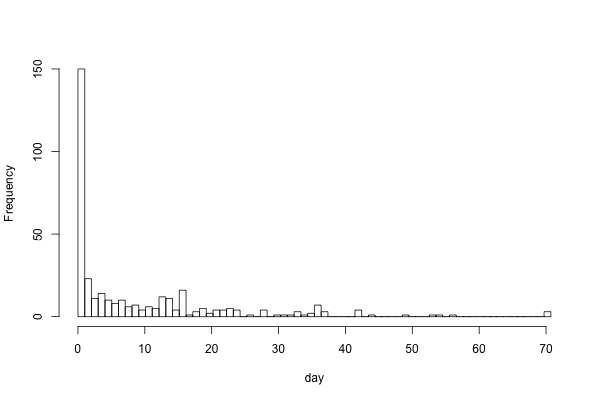
\includegraphics[width=9cm]{../AprilProject/pic/distribution/issue duration distribution total.png}
    \caption{Duration of Issues Distribution across all Teams}
    \label{issue_duration_total}
\end{figure}

While the overall picture of issue duration was very telling, we wanted to focus on the individual groups as well. Figure \ref{issue_duration_team1} focuses on the distribution of issues for team 1. Surprisingly, zero days was not the dominant figure on this distribution, but rather most issues remained open for a day. The differences here compared to the entire class seems to indicate that, at least for team 1, issues were actually being posted then later resolved, rather than being posted after the fact. The distribution for team 1 certainly looks healthier than the overall class.

\begin{figure}[H]
    \centering
    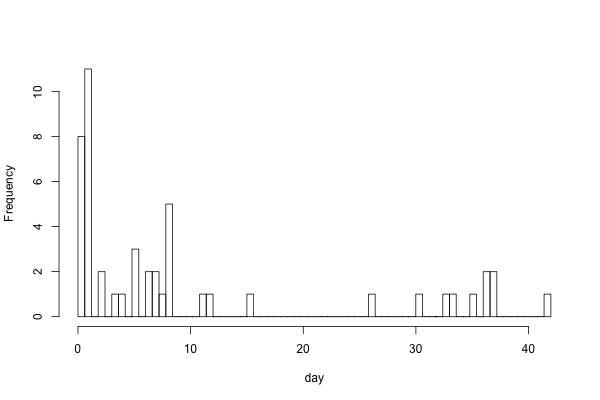
\includegraphics[width=9cm]{../AprilProject/pic/distribution/issue duration distribution team1.png}
    \caption{Duration of Issues Distribution for Team 1}
    \label{issue_duration_team1}
\end{figure}

Once again, team 2 seems to have more unhealthy behavior as seen in figure \ref{issue_duration_team2}. The overwhelming majority of team 2's issues were closed within the same day. There were a couple left open for longer and some even after the 20 day healthy threshold. This behavior seems to imply either very fast development work or that they created issues after the fact to satisfy classroom requirements. 

\begin{figure}[H]
    \centering
    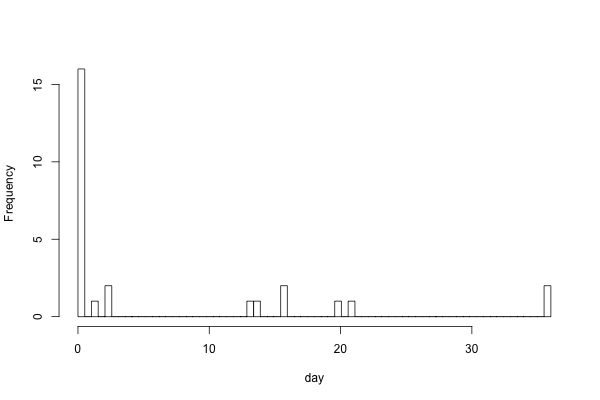
\includegraphics[width=9cm]{../AprilProject/pic/distribution/issue duration distribution team2.png}
    \caption{Duration of Issues Distribution for Team 2}
    \label{issue_duration_team2}
\end{figure}

The most healthy distribution for issue duration was team 3. In figure \ref{issue_duration_team3} team 3 had a fairly even spread of issues from 0 to 20 days and a few forgotten issues closed long past 2 days. This behavior on the issues seems to accurately reflect a cycle of agile development where issues were mostly opened and closed in the span of a couple of weeks. Lining up with different iterations. This is by far the best sign of good development practices across the entire class and the more focused distributions of team 1 and 2. 

\begin{figure}[H]
    \centering
    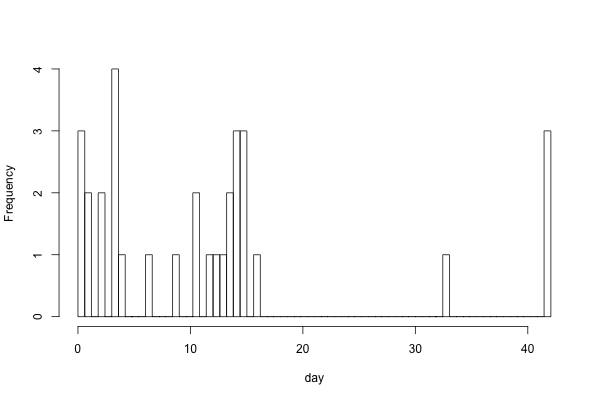
\includegraphics[width=9cm]{../AprilProject/pic/distribution/issue duration distribution team3.png}
    \caption{Duration of Issues Distribution for Team 3}
    \label{issue_duration_team3}
\end{figure}

Overall, issue distribution seems to be a good indicator of the health of a group. When there are plenty of issues that are closed in under 20 days it is a good bet that the team are addressing the problems and closing them in a timely manner. All of the teams had some issues that remained open more than 30 days, but those issues could have been more big picture problems or just issues that slipped through the cracks throughout the development cycle. Team 3 seems to have had the best performance on the issue duration metric with a good spread of issue duration, while keeping the majority of their issues resolved in under 20 days. 

\subsection{Comments vs Issue Duration}
While we predicted that there would be a relationship between comments and issue length it turns out that it is not the case as seen in figure \ref{comments_duration_all}. We targeting all of the teams in the course to try to capture as much data as possible for a more accurate analysis There could be a few different explanations as to why the data does not reflect our hypothesis. One theory is that there were many more older, forgotten, issues that have remained open for much longer than they should have been. Since this was a classroom environment and not a workplace it was hard to enforce rules about issues to keep everything tidy. If a group did not feel like they had to follow the rules, or if they had a different set of rules than everyone else then the data will become skewed. We also noticed that a lot of the high comment issues closed in around 20 days or less. We theorize that these may have been some kind of discussion thread to discuss next steps. 
\begin{figure}[H]
    \centering
    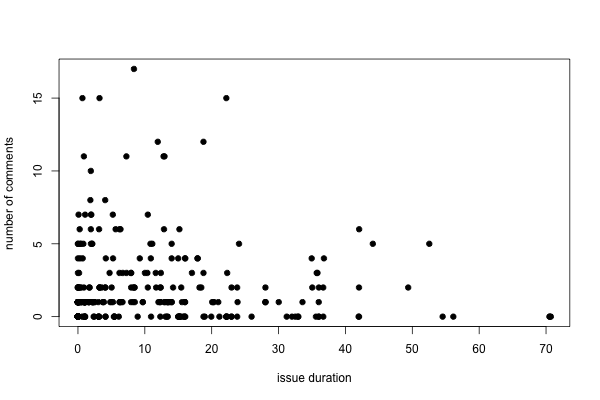
\includegraphics[width=9cm]{../AprilProject/pic/comments_and_issue_duration_all.png}
    \caption{Comments by Issue Duration All Teams}
    \label{comments_duration_all}
\end{figure}

When we were unable to gather any insight out of the overall group data we decided to focus on the three teams instead to see if they had a different story from the overall group. First we pulled the data for team 1, shown in figure \ref{comments_duration_1}. Upon close examination it seems that team 1's data tells the same story as the overall data. The issues with the highest comment counts were all closed in under 15 days, leading us to believe that these were discussion threads. Overall the typical issues seems to only have a handful of comments no matter how long it is open. Once again we think that any issue that was over 25 days old may have been abandoned and later closed as part of a cleanup. 

\begin{figure}[H]
    \centering
    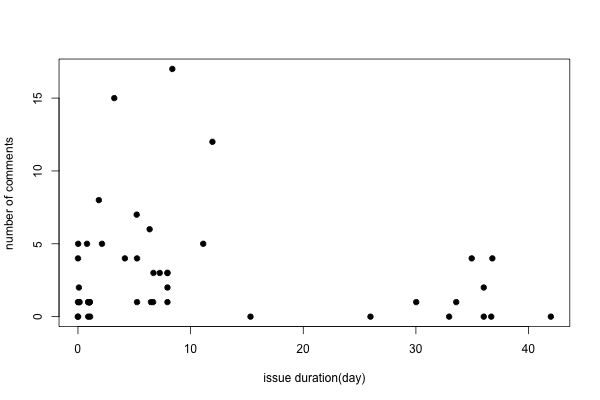
\includegraphics[width=9cm]{../AprilProject/pic/comments_and_issue_duration1.png}
    \caption{Comments by Issue Duration Team 1}
    \label{comments_duration_1}
\end{figure}

Out of all the comments vs issue duration data we pulled, the second team was the most interesting, shown in figure \ref{comments_duration_2}. No matter how long an issue was open it never obtained more than one comment. It seems that there were minimal discussions occurring on GitHub and it almost guarantees that outside communication was occurring for this group. This is perhaps the best insight we can gather from this data. Otherwise, like the others there is no relationship between the issue duration and the number of comments. 

\begin{figure}[H]
    \centering
    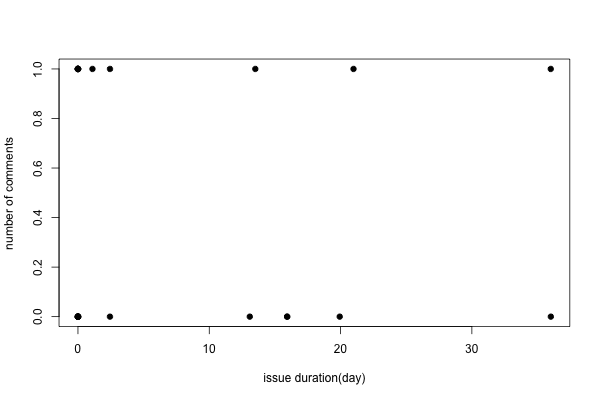
\includegraphics[width=9cm]{../AprilProject/pic/comments_and_issue_duration2.png}
    \caption{Comments by Issue Duration Team 2}
    \label{comments_duration_2}
\end{figure}

The data for team 3 is very similar to the overall data as well as team 1's data, as seen in figure \ref{comments_duration_3}. Most of the issues with more comments were closed under 20 days and there were very few left open for longer than that. Leading us to believe they were forgotten about and later closed. It seems that team 1 and 3 reflect a more typical behavior when it comes to issue duration versus the number of comments. That behavior being that there is not much of a relationship to speak of. 

\begin{figure}[H]
    \centering
    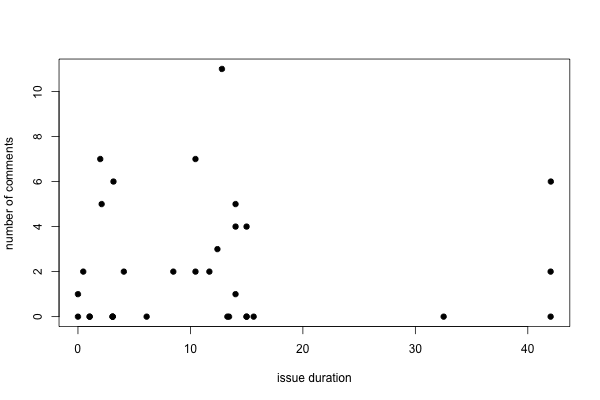
\includegraphics[width=9cm]{../AprilProject/pic/comments_and_issue_duration3.png}
    \caption{Comments by Issue Duration Team 3}
    \label{comments_duration_3}
\end{figure}

Overall, we felt that this metric may not be the best way to analyze the health of a development group since the data did not match up with our predictions. We were able to capture some insight out of the data, especially for team 2 and their lack of comments, but it was not enough to conclude anything about the well being of any group. 


\subsection{Issues closed outside of milestone due date}
When observing the issue close date in reference to its milestone we were not very surprised by the results. The median issue was closed on the milestone due date with many of them being closed before the due date. The habits of team 2 and 3 tended to close most or almost all of their issues on the deadline of the associated milestone. Most likely as a way to clean things up after finishing that particular milestone. Team 1 had a much more varied level of issue close dates. Team 1 had most of it's issues closed before a milestone due date, however there were a good number of which that were closed after the milestone was due. 

\begin{figure}[H]
    \centering
    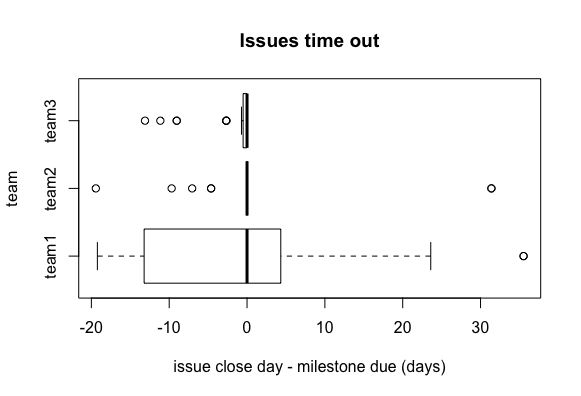
\includegraphics[width=9cm]{../AprilProject/pic/issues_timeout.png}
    \caption{Issue Timeout}
    \label{issue_timeout}
\end{figure}


Except for a few outlier issues that were closed long after the milestone due date, all of the teams were pretty healthy regarding this metric. Based off of the data in figure \ref{issue_timeout} we think that issues were not often closed in a timely manner or the groups were big on procrastinating until the deadline. 


\subsection{Milestone Timeline}

While observing the milestone timeline it was observed that out of the three teams, Team3 did not create enough issues throughout the project and did not set due dates for those milestones as well which is quite different to what was observed for the other two teams. 


\begin{figure}[H]
    \centering
    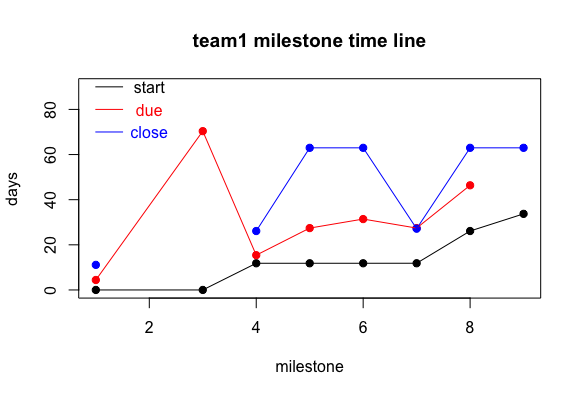
\includegraphics[width=9cm]{../AprilProject/pic/team1_milestone_time.png}
    \caption{Team 1 Milestone Time}
    \label{team1_milestone_time}
\end{figure}

Team1 created the most milestones and set a due date for almost all of them. Team2 as well created milestones throughout the project and set due dates for them.



\begin{figure}[H]
    \centering
    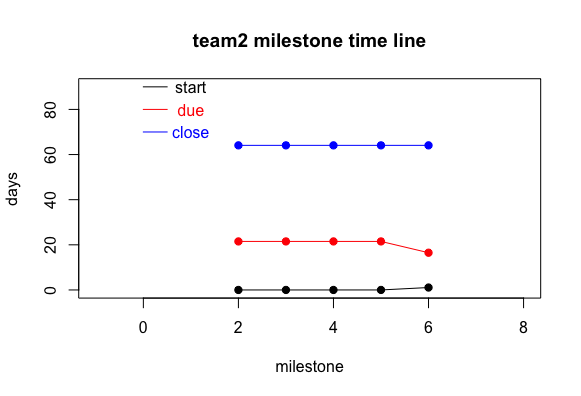
\includegraphics[width=9cm]{../AprilProject/pic/team2_milestone_time.png}
    \caption{Team 2 Milestone Time}
    \label{team2_milestone_time}
\end{figure}


Regarding the closing time of the milestones across all teams it was observed that almost all milestones were closed after the due date set for them. For team 1, only one milestone was closed. Team 1 and 2 closed almost all of their milestones.

\begin{figure}[H]
    \centering
    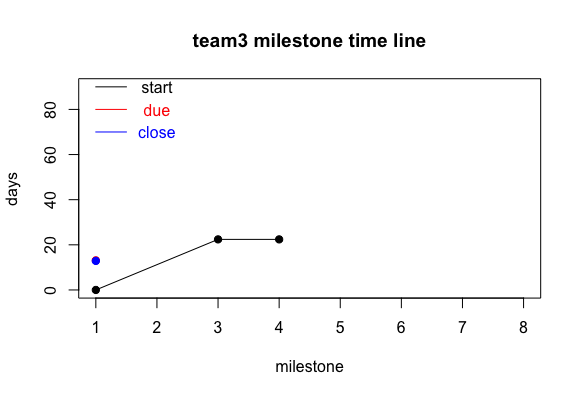
\includegraphics[width=9cm]{../AprilProject/pic/team3_milestone_time.png}
    \caption{Team 3 Milestone Time}
    \label{team3_milestone_time}
\end{figure}


\subsection{Issues assigned to member having comments}


\begin{figure}[H]
    \centering
    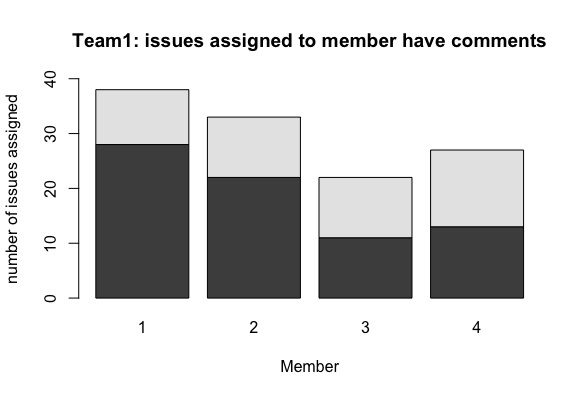
\includegraphics[width=9cm]{../AprilProject/pic/team1_user_issue_comments.png}
    \caption{Team 1 User Issue Comments}
    \label{team1_issue_comment}
\end{figure}

\begin{figure}[H]
    \centering
    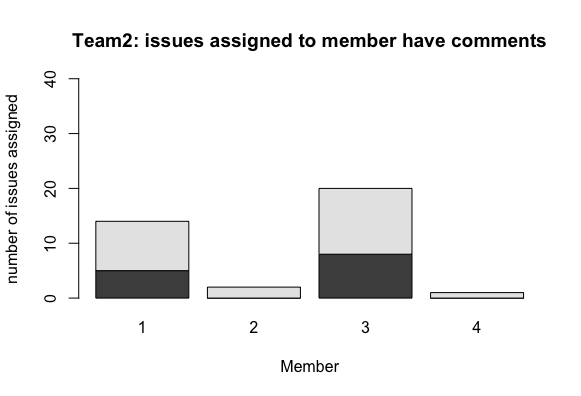
\includegraphics[width=9cm]{../AprilProject/pic/team2_user_issue_comments.png}
    \caption{Team 2 User Issue Comments}
    \label{team2_issue_comment}
\end{figure}

\begin{figure}[H]
    \centering
    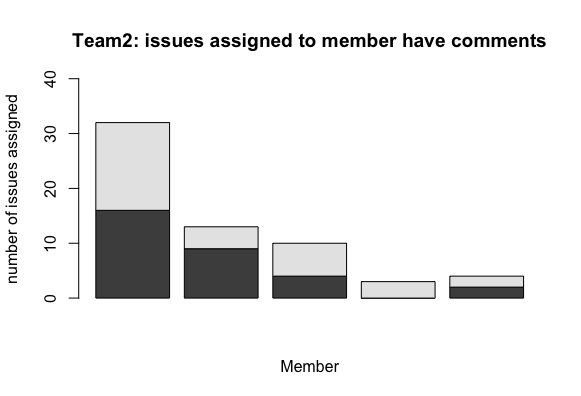
\includegraphics[width=9cm]{../AprilProject/pic/team3_user_issue_comments.png}
    \caption{Team 3 User Issue Comments}
    \label{team3_issue_comment}
\end{figure}

\subsection{Percent commits by user}
When observing the percent commits by the users, it was seen that in none of the three teams the number of commits between the users were balanced. The number of commits can provide a direct correlation with the contribution made by the users but a better metric for contribution could be the number of lines committed. So, it could have happened that the users could have made a few commits but would have committed more lines of code thereby making their contribution more than what meets the eye. But, if we do a deeper analysis it can also be observed that the number of lines could also be a superficial metric to measure contribution of a team member, it could also happen that the functionality implemented by a member could have been difficult to implement and although it took less number of lines to implement it took more time to implement and someone who wrote more lines of code could have been implementing an easy functionality, but then again easy and difficult are subjective to the people implementing it and something which seems difficult to someone could be easy for someone else. 

Here out of the three teams only team1 had commits from all the members and team2 and team3 had one and two members respectively who did not make any commits. This goes on to show their lack of participation in the project. Also, in all the three teams it was observed that there was one person who 


\begin{figure}[H]
    \centering
    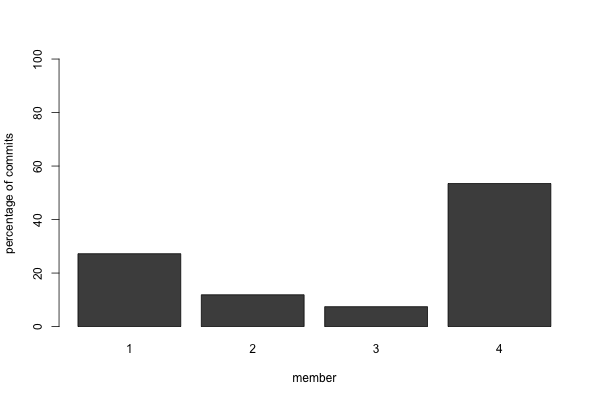
\includegraphics[width=9cm]{../AprilProject/pic/users commit percentage team1.png}
    \caption{Team 1 Percent of Commits by User}
    \label{team1_percent_commit}
\end{figure}

\begin{figure}[H]
    \centering
    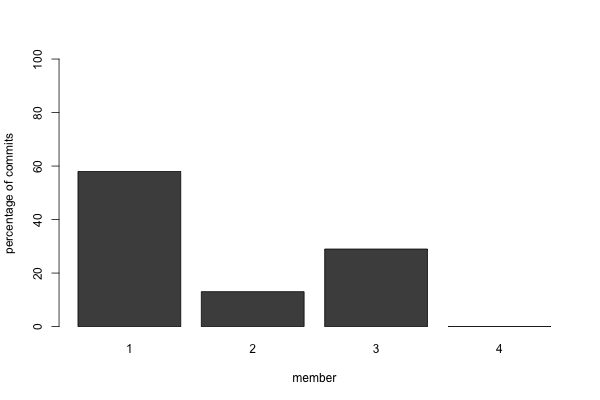
\includegraphics[width=9cm]{../AprilProject/pic/users commit percentage team2.png}
    \caption{Team 2 Percent of Commits by User}
    \label{team2_percent_commit}
\end{figure}

\begin{figure}[H]
    \centering
    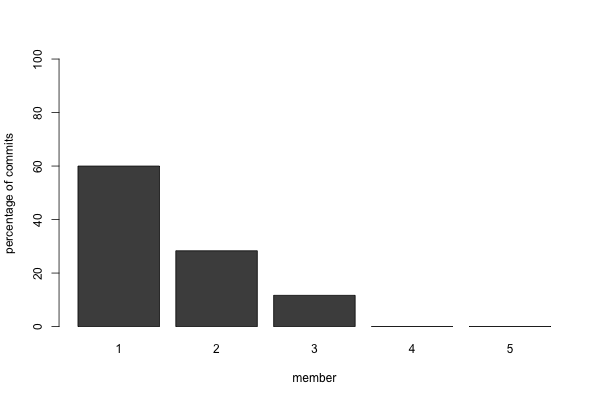
\includegraphics[width=9cm]{../AprilProject/pic/users commit percentage team3.png}
    \caption{Team 3 Percent of Commits by User}
    \label{team3_percent_commit}
\end{figure}

\section{Bad Smells Detector}
\section{Early Warning}

\end{document}